\chapter{State of the Art}
\label{chap:stateofart}

This chapter introduces a modest literature review regarding \gls{IoT}.
Following this two themes some related technologies are briefly presented and then compared.
The intent of this chapter is to introduce the reader to the subjects related to this work.

\section{Internet of Things}
\label{sec:stateofart:iot}

\section{IoT Architectural Context}
\label{sec:stateofart:arch}

\subsection{Infrastructure}
\label{subsec:stateofart:arch:infra}

\subsubsection{Message Broker}
\label{subsubsec:stateofart:arch:infra:broker}

\subsubsection{IoT Midlleware}
\label{subsubsec:stateofart:arch:infra:middleware}

\subsubsection{Asynchronous Communication}
\label{subsubsec:stateofart:arch:infra:async}

\subsubsection{Data Storage}
\label{subsubsec:stateofart:arch:infra:store}

\subsubsection{Rule Engine}
\label{subsubsec:stateofart:arch:infra:rule}

\subsection{Platforms}
\label{subsec:stateofart:arch:platforms}

\subsection{Solutions}
\label{subsec:stateofart:arch:solutions}

\subsection{Reference Architectures}
\label{subsec:stateofart:arch:ref}

\subsubsection{IoT ARM}
\label{subsubsec:stateofart:arch:arm}

\subsubsection{IIRA}
\label{subsubsec:stateofart:arch:iira}

\subsubsection{WSO2 IRA}
\label{subssubsubsecec:stateofart:iot:wso2}

\subsubsection{Intel SAS}
\label{subsubsec:stateofart:arch:intel}

\subsubsection{Azure IRA}
\label{subsubsec:stateofart:arch:azure}

\subsubsection{SAT-IoT}
\label{subsubsec:stateofart:arch:sat}

\subsection{Synopsis}
\label{subsec:stateofart:arch:synopsis}

\section{Business Areas}
\label{sec:stateofart:areas}

Even though there's no concise structure, it is obvious that the \gls{IoT} technologies can be used in a broad range of areas/sectors. According to \cite{nivzetic2019smart}, the most valuable areas are: Smart Cities, Industrial \gls{IoT}, Connected Health and Smart Homes. The general market division of IoT technologies is presented in Figure~\ref{fig:iot-areas}.

\begin{figure}[H]
    \centering
    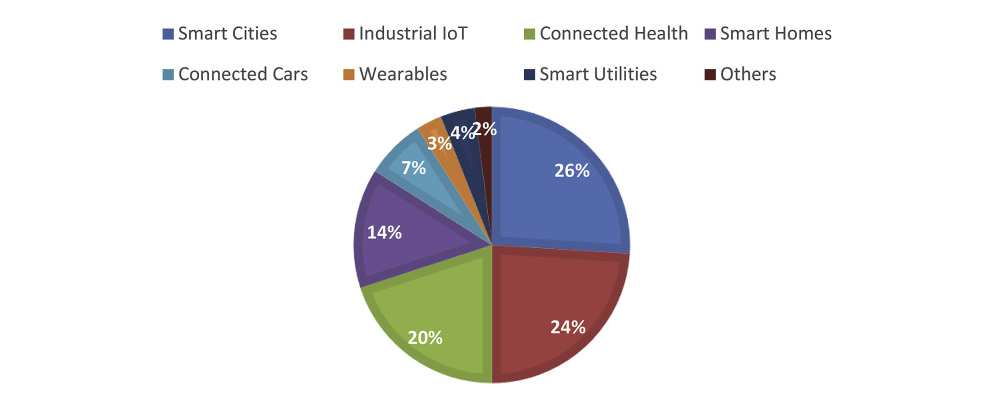
\includegraphics[scale=0.5]{
        assets/figures/iot-areas.png
    }
    \caption[IoT market structure]{General market structure of IoT technologies, \cite{nivzetic2019smart}}
    \label{fig:iot-areas}
\end{figure}

From another point of view, and according to \cite{7073822}, the sectors \gls{IoT} is related to are: Energy, Smart City, Transportation, Smart Home, Environment, Supply Chain, and Health Care.

According to (\cite{6851114}) these are the main application fields for \gls{IoT} in China: industry, smart agriculture, smart logistics, intelligent transportation, smart grids, smart environmental protection, smart safety, smart medical and smart home.

Even though this work focus mostly on Smart Cities other areas will also be described. Each of this areas incorporate several interconnected use cases that will briefly described in the following segments in accordance with \cite{nivzetic2019smart}.

\subsection{Smart Cities}
\label{subsec:stateofart:areas:cities}

The Smart Cities sector includes numerous use cases related to public safety, the environment, mobility, energy, infrastructure and many other municipal concerns. According to \cite{iot-smart-city-prioritized} this are the use cases being prioritized.

\begin{itemize}
    \item Connected Public Transport: real-time monitoring of public transportation vehicles' locations, stops and itineraries, and the possibility to be notified when a public transportation vehicle is arriving at a stop;
    \item Traffic Monitoring and Management: real-time monitoring and management of traffic flows in a efficient manner;
    \item Water level / Flood Monitoring: real-time monitoring of level of water in public water basins such as rivers, channels, or even lakes and seas to warn and predict fast water level shifts;
    \item Video Surveillance \& Analytics: real-time monitoring using \gls{CCT} cameras and analytics to detect specific situations, e.g. accidents, crimes, potential threats, or recognize specific features (face recognition, demographics, etc.);
    \item Connected Streetlights: real-time monitoring and management of streetlights' health status and energy consumption to decrease costs and become more sustainable;
    \item Weather Monitoring: real-time monitoring of weather conditions such as temperature, humidity, rainfall, wind speed and direction to predict the weather and future natural disasters;
    \item Air Quality / Pollution Monitoring: real-time monitoring of air quality to warn the community about hazardous conditions;
    \item Smart Metering - Water: remote real-time monitoring of water usage in homes to address the world's water demand and scarcity issues and faster localize sewage leaks;
    \item Fire / Smoke Detention: real-time monitoring of possible indoor fires and CO2 levels to prevent injuries, fatalities and building degradation;
    \item Water Quality Monitoring: real-time monitoring of water conditions such as pH levels, percentage of salts and other elements that can threaten the public health.
\end{itemize}

Apart from these use cases, others are arising, such as smart parking (\cite{GOAP201841}), smart irrigation (\cite{7562735}) and waste management (\cite{7972276}).
\begin{itemize}
    \item Smart parking provides a simple method to the community of knowing the available parking spots, which, alone, lowers the carbon footprint and traffic congestions in cities.

    \item Smart irrigation tackles the need to save water by irrigating the soil only when needed and not when it is already moist, it's raining or it is expected to rain in the following hours.

    \item Waste management can eliminate the cost of unnecessary waste collections and therefore reduce the carbon footprint. Data gathered can then help to identifying cost-effective itineraries to collect waste and eventually lower overall transportation and staff costs.
\end{itemize}

All this use cases refine the efficiency of the municipal workforce and help the town council to reduce costs and improve the environment sustainability in the long term.

\subsection{Industry}
\label{subsec:stateofart:areas:industry}

According to \cite{iiot}, ``the Industrial \gls{IoT} provides a way to get better visibility and insight into the company's operations and assets", therefore this leads to ``operational efficiency gains and accelerated productivity, which results in reduced unplanned downtime and optimized efficiency, and thereby profits"".
It is comprised of several use cases (\cite{iiot-cases}) such as:

\begin{itemize}
    \item Predictive Maintenance: real-time monitoring of equipment conditions and applied data analytics can help a company to significantly decrease operational expenditures. ``Other potential advantages include increased equipment lifetime, increased plant safety and fewer accidents with negative environmental impact"" (\cite{iiot-cases});
    \item Smart metering: real-time monitoring of energy, water or natural gas consumption of a building can reduce operating expenses by managing manual operations remotely, reduce energy theft and improve forecasting and streamline power-consumption (\cite{metering-sierra});
    \item Asset tracking: real-time monitoring of resources helps "to easily locate and monitor key assets, along the supply chain (e.g. raw materials, final products and containers) to optimize logistics, maintain inventory levels, prevent quality issues and detect theft" (\cite{iiot-cases}).
    \item Connected vehicles: computer-enhanced vehicles that automate many normal driving tasks can lower crash rates, and help decreasing the number of vehicles a company needs to function.
    \item Fleet management: real-time monitoring of vehicles location and conditions can help ``improving efficiency and productivity while reducing overall transportation and staff costs"" (\cite{iiot-cases}).
\end{itemize}

As we can see from the list above, the Industrial \gls{IoT} sector is focused on business efficiency and staff safety, which, as a side effect, brings environmental benefits.

\subsection{Healthcare}
\label{subsec:stateofart:areas:healthcare}

According to \cite{FIROUZI2018583} new opportunities are now arising as a result of fast-paced expansion in the areas of the \gls{IoT} and Big Data for healthcare industries. People across the globe have begun to adopt wearable biosensors, whose data is feed into the new emerging individualized health applications.
This sector incorporates numerous use cases (\cite{iot-healthcare}) such as:

\begin{itemize}
    \item Remote Healthcare Monitoring: real-time monitoring of a patient conditions such as pulse rate and heartbeat can prevent unwanted deaths;
    \item Drug management: medicine monitoring and reminder system can help the elderly to take medicine on time;
    \item Employee health management: real-time monitoring of employee's state can predict burnouts and increase a workforce productivity;
\end{itemize}

The benefits these use cases provide are a more convenient lifestyle, improvement of one life's quality, reduction in costs and increased survival rates of patients (\cite{iot-healthcare}).

\subsection{Smart Homes}
\label{subsec:stateofart:areas:home}

Visions of smart homes have long caught the attention of researchers and considerable effort has been put toward enabling home automation. However, these technologies have not been widely adopted despite being available for over three decades (\cite{iot-smarthomes}).
Based on \cite{smarthome-review} most home automation services offer the following use cases:

\begin{itemize}
    \item Smart Lighting: remote and automated control of lights inside a house can help to decrease energy wasted;
    \item Smart Air Conditioning: remote and automated control of air conditioners can keep the house comfortable while minimizing the energy wasted;
    \item Remote health monitoring: when dealing with the elderly, complex smart systems can anticipate their needs without direct human intervention;
    \item Device Automation: smart systems can turn the lights off when no one is home, open the door when an identified person arrives and must more, improving the overall comfort of the residents.
\end{itemize}

A smart home delivers various benefits such as reducing energy waste, comfort, allowing remote control of the house, monitoring of elderly patients and easy communication with health institutions (\cite{smarthome-review}).

\subsection{Open Challenges}
\label{subsec:stateofart:arch:challenges}

Even though it seems \gls{IoT} is the obvious next step for the industry, healthcare, everyone's home, public spaces/services and everything else there are some obstacles to overcome.

One of the big challenges ahead of everyone is related with antiquated ideas, tools and processes still in use today.
Each of the use cases above mentioned require a big shift in how a company works since it demands a modernization of the organization infrastructure.
\cite{tapscott2006wikinomics}, explained that ``In an age where mass collaboration can reshape an industry overnight, the old hierarchical ways of organizing work and innovation do not afford the level of agility, creativity, and connectivity that companies require to remain competitive in today's environment"".

According to \cite{7073822} this are the most important challenges regarding \gls{IoT} applications:

\begin{itemize}
    \item Technological Interoperability: achieving a seamless interaction between devices and people with devices (according to \cite{al2016iot} there's a lack of standardization in \gls{IoT} devices and technologies);
    \item Semantic Interoperability: guaranty that the devices interpret the shared information
correctly and act accordingly (improvements have to be made regarding distributed ontologies, semantic web, or semantic device discovery);
    \item Security and Privacy: improving data integrity, unique device identification, encryption and implement proper data/device ownership for legal/liability issues;
    \item Smart Things: ultra low power circuits and devices capable of tolerating harsh environments have to be developed;
    \item Resilience and Reliability: in industrial environments or in emergency use cases temporary outages cannot be accepted.
\end{itemize}

According to the author this challenges substantially lingered the growth of \gls{IoT}, an area that was expected to have a much bigger impact in day-to-day life of everyone. According to \cite{iot-cisco-prediction} there would be 50 billion of devices connected to the Internet by 2020 but \cite{statista-number-devices} reported only 8.74 billion of connected devices.

\cite{noura2019interoperability} introduced more issues in \gls{IoT} related to interoperability from different perspectives:

\begin{itemize}
    \item Device interoperability: concerned with the exchange of information between heterogeneous devices and the ability to integrate new devices into any \gls{IoT} platform;
    \item Network interoperability: concerned with information addressing, routing, security, resource optimization, \gls{QoS} and mobility support;
    \item Syntactical interoperability: concerned with the format and structure of the information exchanged between heterogeneous systems;
    \item Semantic interoperability: concerned with the meaning behind the information exchanged, heterogeneous devices can, for example, work with diverse unit measurements;
    \item Platform interoperability: concerned with heterogeneous platforms that use diverse programming languages, \gls{OS} and software architectures.
\end{itemize}

For \gls{IoT} Technologies to deliver on the promises made by companies like Cisco or Gartner, these barriers must be surpassed.

\section{Synopsis}
\label{sec:stateofart:synopsis}

This chapter presented the big theme surrounding this work: \gls{IoT}.

In the \gls{IoT} section some business cases relevant for this work were introduced. Besides these, several solutions currently in the market were presented.
The technologies usually used to tackle the challenges related to \gls{IoT} were presented in the \nameref{sec:stateofart:tech} section, these were: (i) Asynchronous Communication, (ii) Data Processing and (iii) Data Storage.

In the following chapter, \nameref{chap:requirements}, some of the business cases and challenges discussed here will be tackled.
